% \documentclass[a4paper, 12pt]{article}
% \usepackage{header}

% \begin{document}
% \pagestyle{fancy}

\section{Лекция 8 от 11.10.2016. Сегментация и кластеризация изображений
с помощью потоковых алгоритмов}

\subsection{Постановка задачи}

Рассмотрим любую картинку (Айрат, привет):

\begin{figure}[H]
  \center{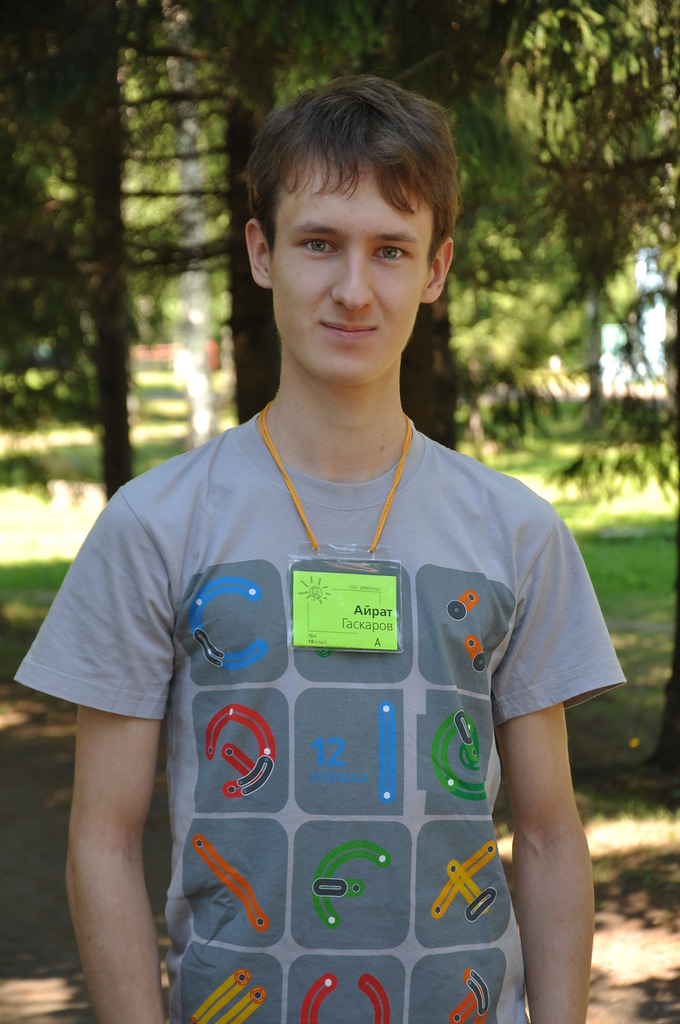
\includegraphics[width=0.5\linewidth]{../images/Airat.jpg}}
  \caption{Произвольная картинка}
\end{figure}

И мы хотим отделить фон от человека. То есть присвоить каждому пикселю матрицы
$n \times m$ какой-то label, к какому классу относится --- фон или человек,
например.

Фактически это единственный алгоритм машинного обучения, где используются
алгоритмы на потоках.

\textit{Прим. Те, кто не помнят, что такое поток, могут закрывать эту лекцию.}

\subsection{Минимизация парно-сепарабельной энергии от бинарных переменных}

Пусть у нас задан неориентированный граф $G(V, E)$. Для каждого $i \in V$ пусть
$x_i$ могут принимать значения только из $\{0, 1\}$.

\begin{Def}
  Назовём \textbf{энергией} (обозначение $I$) функцию из $\{0, 1\}^{|V|} \to
  \R$:
  \[
    I(X) = \sum_{i \in V} \theta_i(x_i) + \sum_{(i, j) \in E} \theta_{ij}(x_i, x_j) +
    \theta_0,
  \]

  где $\theta_i, \theta_{ij}$ --- какие-то потенциалы, а $\theta_0$ --- константа.
\end{Def}

И наша задача заключается в том, что минимизировать $I(X)$. Известно, что если
не вводить никаких дополнительных ограничений, то задача минимизации 
энергии является $\NPclass$-трудной.

Давайте поймём, как
это относится к сегментации. На выборке из огромного числа изображений мы
можем с уверенностью говорить, о том, какие пиксели находятся рядом, какие
далеко по цвету, поэтому можем поставить какие-то веса на рёбрах. После этого
сегментировать изображение, чтобы были в одной и другой части как можно
более тёплые цвета. Рассмотрим частный случай потенциалов, в котором задача
становится полиномиальной:

\begin{itemize}
  \item $\forall \ i \in V, \theta_i(0) \geqslant 0, \theta_i(1) \geqslant 0$;
  \item $\forall \ (i, j) \in E \Rightarrow \theta_{ij}(0, 0) = \theta_{ij}(1, 1) = 0, 
  \theta_{ij}(0, 1) \geqslant 0, \theta_{ij}(1, 0) \geqslant 0$.
\end{itemize}

Тогда энергию можно задать так (легко проверить все случаи):

\[
  I(X) = \sum_{i \in V} (x_i\theta_i(1) + (1 - x_i)\theta_i(0)) + 
  \sum_{(i, j) \in E} (x_i(1 - x_j)\theta_{ij}(1, 0) + 
  x_j(1 - x_i)\theta_{ij}(0, 1)) + \theta_0,
\]

\begin{figure}[H]
  \center{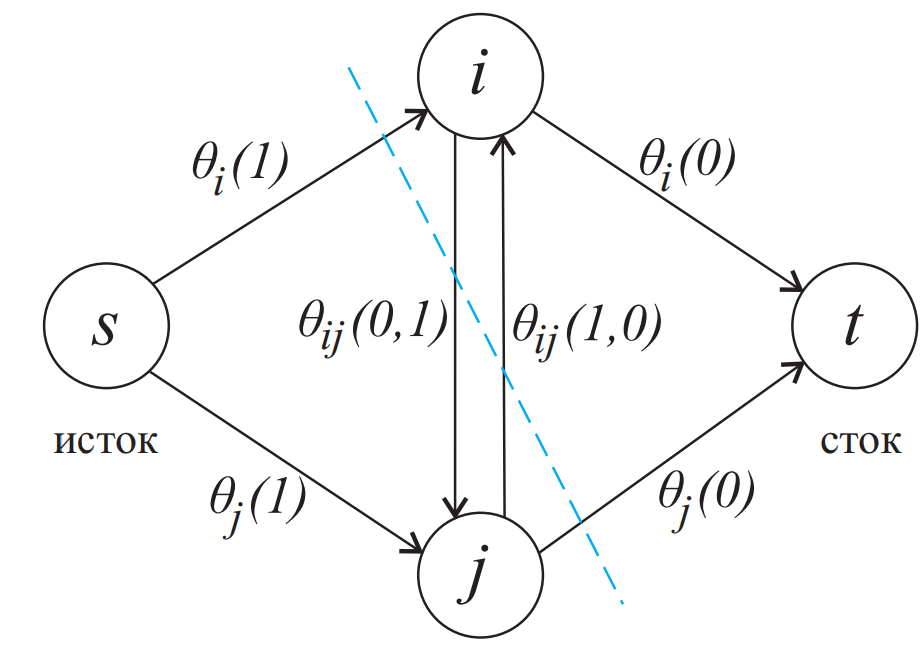
\includegraphics[width=0.5\linewidth]{../images/graph.png}}
  \caption{Граф, построенный для минимизации энергии от двух переменных
  $x_i, x_j$. Разрез, отображенной пунктирной линией соответствует присваиванию 
  $x_i = 1, x_j = 0$. Величина разреза составляет $\theta_i(1) + \theta_j(0) +
  \theta_{ij}(1, 0)$}.
\end{figure}

Теперь построим ориентированный граф $\overline{G} = (\overline{V}, \overline{E})$
по следующим правилам:

\begin{itemize}
  \item В $\overline{V} = V \cup \{s, t\}$;
  \item Неориентированные рёбра делаем ориентированными в обе
  стороны, а для каждой вершины
  $i$ проведем ещё ребра $(s, i), (i, t)$;
  \item $c(s, i) = \theta_i(1), c(i, t) = \theta_i(0)$, где $i \in V$;
  \item $\forall \ (i, j) \in E$ таким, что $i < j$ положим $c(i, j) =\theta_{ij}(0, 1), c(j, i) = \theta_{ij}(1, 0)$;
  \item Все вершины из $V$, которые попали в минимальный разрез $S$ положим $x_i = 0$,
  остальным $x_i = 1$.
\end{itemize}

Тогда видно, что минимизация разреза эквивалентна этой задаче, что эквивалентно
задаче максимального потока. Существует, конечно, много алгоритмов максимального
потока, многие из них мы изучали, но в компьютерном зрении часто возникают алгоритмы
Бойкова-Колмогорова и IBFS. С ними вы можете ознакомиться при желании самостоятельно.

Пример графа, построенного для энергии от 2-х переменных, и его разреза 
приведен на рис 2.

\subsection{Репараметризация}

Здесь мы рассмотрим, какие ещё энергии можно минимизировать при помощи
разрезов графов. Назовём преобразования потенциалов, не меняющее энергию 
\textit{репараметризацией}. Рассмотрим несколько видов репараметризаций:

\begin{itemize}
  \item Вычитание константы --- $\theta_i(0) \mathrel{{-}{=}} \delta, \theta_i(1) \mathrel{{-}{=}} \delta,
  \theta_0 \mathrel{{+}{=}} \delta$;
  \item Изменение потенциалов на ребрах. $\theta_{ij}(p, 0) \mathrel{{-}{=}} \delta, 
  \theta_{ij}(p, 1) \mathrel{{-}{=}} \delta, \theta_i(p) \mathrel{{+}{=}} \delta$. Аналогично, если
  $p$ на 2-ой координате.
\end{itemize}

Легко видеть из определения, что эти преобразования не меняют энергию.

Рассмотрим, что можно делать при помощи репараметризации потенциалов на ребрах.
Для $(i, j) \in E$ пусть 
$\theta_{ij}(0, 0) = a$,
$\theta_{ij}(1, 1) = b$,
$\theta_{ij}(0, 1) = c$,
$\theta_{ij}(1, 0) = d$.

После этого давайте 3 раза применим 2-ой пункт видов репараметризации:

\begin{itemize}
  \item $\theta_{ij}(0, 0) \mathrel{{-}{=}} a, \theta_{ij}(0, 1) \mathrel{{-}{=}} a, \theta_{i}(0) \mathrel{{+}{=}} a$;
  \item $\theta_{ij}(0, 1) \mathrel{{-}{=}} (c - a), \theta_{ij}(1, 1) \mathrel{{-}{=}} (c - a),
  \theta_{j}(1) \mathrel{{+}{=}} c - a$;
  \item $\theta_{ij}(1, 1) \mathrel{{-}{=}} (b - c + a), \theta_{ij}(1, 0) \mathrel{{-}{=}} (b - c + a),
  \theta_{i}(1) \mathrel{{+}{=}} b - c + a$
\end{itemize}

Потом сделаем все потенциалы вершины неотрицательными по 1-ому пункту
репараметризации. В итоге у нас ненулевым останется только $\theta_{ij}(1, 0) =
d + c - a - b$. И если оно положительно, то мы можем применить наш алгоритм, то
есть должно выполняться условие \textit{субмодулярности}:

\[
  \theta_{ij}(0, 0) + \theta_{ij}(1, 1) \leqslant \theta_{ij}(0, 1) + 
  \theta_{ij}(1, 0)
\]

Данное условие вызвано тем, что для полиномиальной разрешимости задач о 
максимальном потоке и минимальном разрезе пропускные способности дуг графа
должны быть неотрицательны.

\subsection{$\alpha$-расширение}

Мы умели решать задачу только с одним объектом, теперь давайте попробуем
приближенно решить задачу со многими объектами. Тот же граф, только теперь
поставим в соответствие каждой вершине $i$ --- $y_i \in \{1, \ldots, K\}$ ---
классы разбиения. Рассмотрим следующую энергию:

\[
  I_M(X) = \sum_{i \in V} \psi_i(x_i) + \sum_{(i, j) \in E} \psi_{ij}(x_i, x_j) +
    \psi_0,
\]

Буква $M$, скорее всего, идёт от английского слова Many --- много.

Алгоритм $\alpha$-расширение минимизирует энергию при помощи выполнения шагов между 
разметками $y$, каждый из которых гарантированно не увеличивает значение энергии. 
Каждый шаг
представляет собой задачу минимизации энергии бинарных переменных вида.
Неформально каждый шаг позволяет каждой переменной из $y$ либо присвоить выбранное значение 
$\alpha$, либо оставить текущее значение (расширение метки $\alpha$).

\begin{figure}[H]
  \center{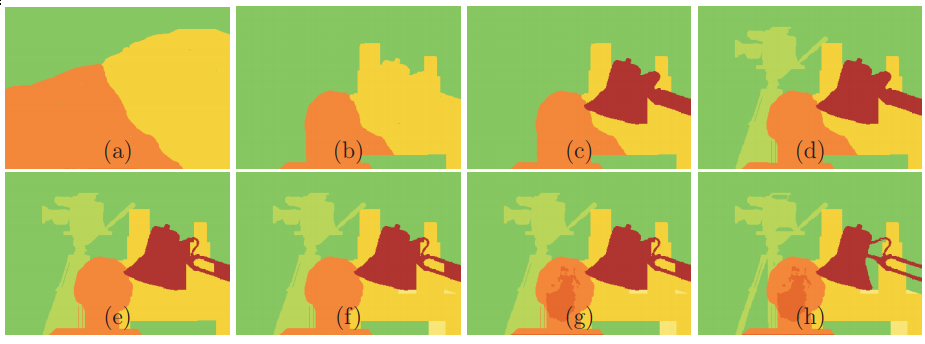
\includegraphics[width=1\linewidth]{../images/alpha.png}}
  \caption{Пример работы алгоритма $\alpha$-расширения для задачи
  выровненного стерео. (a) -- начальная разметка, далее последовательные
  расширения различных меток.}
\end{figure}

На каждом шаге алгоритма у нас есть текущее приближение $y^0$ и выбрана
\textit{расширяемая} метка $\alpha \in \{1, \ldots, K\}$.

\begin{itemize}
  \item Граф, потенциалы сначала одинаковы;
  \item Применяем алгоритм о минимальном разрезе, теперь, если $x_i = 0$, то
  оставляем $y_i^0$, а если $x_i = 1$, то меняем переменную $y_i^0 = \alpha$;
  \item Меняем все потенциалы вершин: $\theta_i(0) = \psi_i(y_i^0), 
  \theta_i(1) = \psi_i(\alpha);$
  \item Меняем потенциалы на ребрах: $\theta_{ij}(0, 0) = \psi_{ij}(y_i^0, y_j^0),
  \theta_{ij}(1, 1) = \psi_{ij}(\alpha, \alpha), \theta_{ij}(0, 1) =
  \psi_{ij}(y_i^0, \alpha), $
  
  $\theta_{ij}(1, 0) = \psi_{ij}(\alpha, y_j^0)$;
  \item Повторяем процедуру, сколько нам надо для реальной задачи.
\end{itemize}

% \end{document}
